%\documentclass[handout]{beamer}
\documentclass[ignorenonframetext]{beamer}
\usepackage[utf8]{inputenc}
\usepackage[german, english]{babel}
\usepackage{lmodern}
\usepackage[T1]{fontenc}
\usepackage{verbatim}
\usepackage{amsmath}
\usepackage{graphicx}
\usepackage{float}
\usepackage{framed}
\usepackage{mathtools}
\usepackage[font=footnotesize]{caption}
\captionsetup{format=hang}
%\usepackage[hyperfigures =true ,linkcolor =black, urlcolor=blue, colorlinks =true, citecolor=black ,pdfauthor ={ Leonard Peter Wossnig}, ={Analytic solution and Monte Carlo simulation of the two dimensional q-state Potts model},pdfcreator ={ pdfLaTeX }]{hyperref}
%\usepackage{braket}pdftitle
%%%\usepackage[dvips]{color}
%\usepackage[pdftex]{graphicx}
%%%\usepackage{subfigure}
\usetheme{Malmoe}
\useoutertheme{infolines}
%\usepackage{mathpazo}
\parskip1.5ex

\newcommand{\changefont}[3]{\fontfamily{#1}\fontseries{#2}\fontshape{#3}\selectfont}



\newcommand{\dif}{\mathrm{d}}


%------------------------------------------------------------------------------------
\title[]{Leaping into Lyapunov Space}
\subtitle{}
\author[Milling, Petzak]{\large{Manuel Milling, Tobias Petzak} \\
}
\institute[Universität Augsburg]{Institut für Physik der Universität Augsburg} 

\date[26.08.2016]

\titlegraphic{
\hspace{1cm}
%\includegraphics[height=2cm]{ekm}
\hspace{1cm}
%\includegraphics[height=2cm]{unia}
\hspace{1cm}
}


\beamertemplatenavigationsymbolsempty

\setbeamertemplate{headline}
{
  \leavevmode%
  \hbox{%
  \begin{beamercolorbox}[wd=1\paperwidth,ht=2.25ex,dp=1ex,left,leftskip=1em]{section in head/foot}%
    \usebeamerfont{subsection in head/foot}\hspace*{2ex}\insertsectionhead
  \end{beamercolorbox}%
  }%
  \vskip0pt%
}
\makeatletter

\setbeamertemplate{footline}
{
  \leavevmode%
  \hbox{%
  \begin{beamercolorbox}[wd=.5\paperwidth,ht=2.25ex,dp=1ex,center]{author in head/foot}%
    \usebeamerfont{author in head/foot}\insertshortauthor~~\beamer@ifempty{\insertshortinstitute}{}{}
  \end{beamercolorbox}%
  \begin{beamercolorbox}[wd=.5\paperwidth,ht=2.25ex,dp=1ex,right]{date in head/foot}%
    \usebeamerfont{date in head/foot}\insertshortdate{}\hspace*{2em}
  \end{beamercolorbox}}%
  \vskip0pt%
}
\makeatother
\begin{document}
\frame[plain]{\titlepage}

\section*{Table of Contents}
\begin{frame}
\frametitle{Table of Contents}
\begin{itemize}
\item Motivation
\item The Logistic Equation
\item The Lyapunov-Exponent
\item Algorithm and Code presentation
\item Pictures
\end{itemize}
\end{frame}

\section*{Motivation}

\begin{frame}
\frametitle{Motivation}
%\begin{itemize}
\begin{center}
\begin{equation}
x \leftarrow rx(1-x)
\end{equation}
$ \Rightarrow$ Jellyfish, The Swallow, Zircon Zity, ....
\end{center}

%\end{itemize}
\end{frame}

\section*{The Logistic Equation}
\begin{frame}
\frametitle{The Logistic Equation}
\begin{tabular}{cr}
\begin{minipage}[t]{0.5\textwidth}
\vspace*{5pt}
\begin{itemize}
\item $x \leftarrow rx(1-x) $
\item Simplest known formula to describe a chaotic dynamic system
\item Can\glqq describe\grqq~animal population
\item Depending on $r$ one-point, two-point, multi-point attractor or chaotic behaviour
\end{itemize}
\end{minipage}


\begin{minipage}[t]{0.4\textwidth}
\begin{figure}[htbp]
\vspace*{5pt}
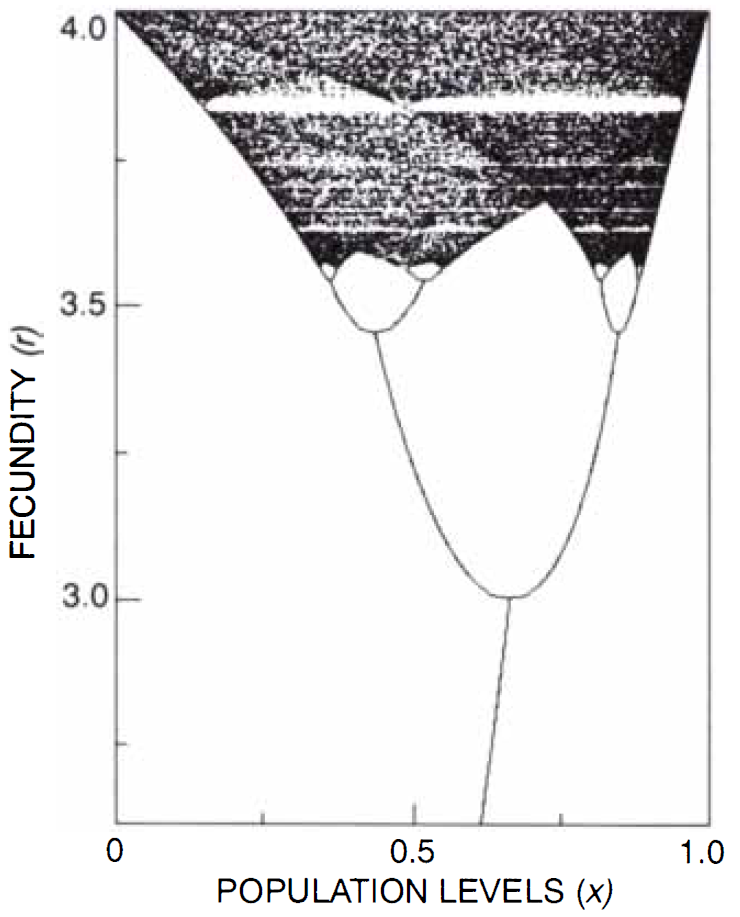
\includegraphics[width = \textwidth]{population}
\end{figure}
\end{minipage}
\end{tabular}
\end{frame}


\begin{frame}
\frametitle{Population Evolution}
\begin{tabular}{cr}
\begin{minipage}{0.4\textwidth}
\begin{figure}[htbp]
\vspace*{-15pt}
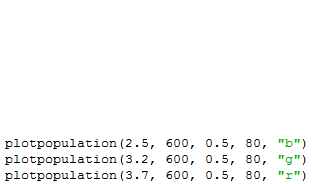
\includegraphics[width = \textwidth]{population-development1-code}
\end{figure}
\end{minipage}

&\begin{minipage}[t]{0.6\textwidth}

\begin{figure}[htbp]
\vspace*{-45pt}
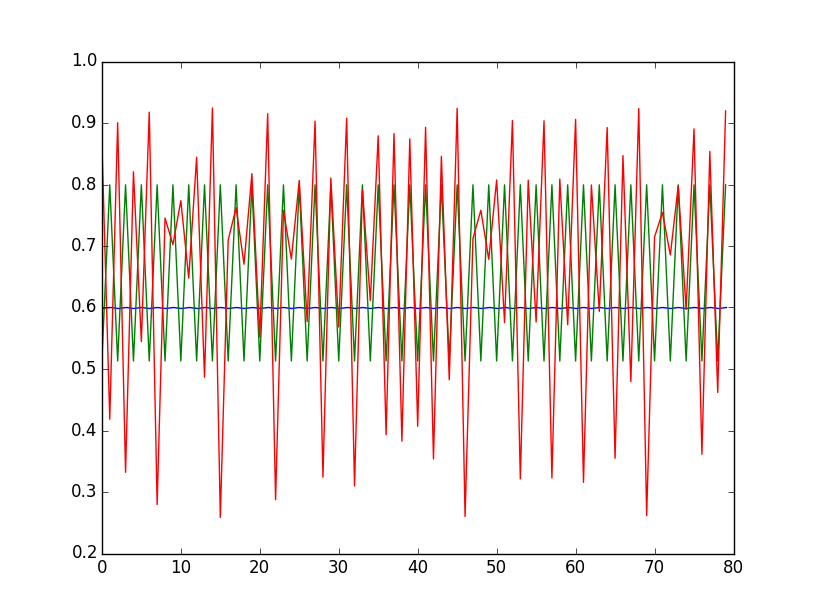
\includegraphics[width = 0.8\textwidth]{population-development1}
\end{figure}
\end{minipage}

\\\begin{minipage}{0.4\textwidth}
\begin{figure}[htbp]
%\vspace*{15pt}
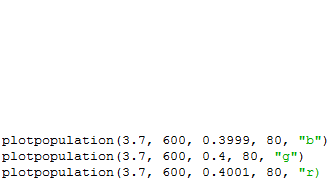
\includegraphics[width = \textwidth]{population-development2-code}
\end{figure}
\end{minipage}

&\begin{minipage}[t]{0.6\textwidth}
\begin{figure}[htbp]
\vspace*{-45pt}
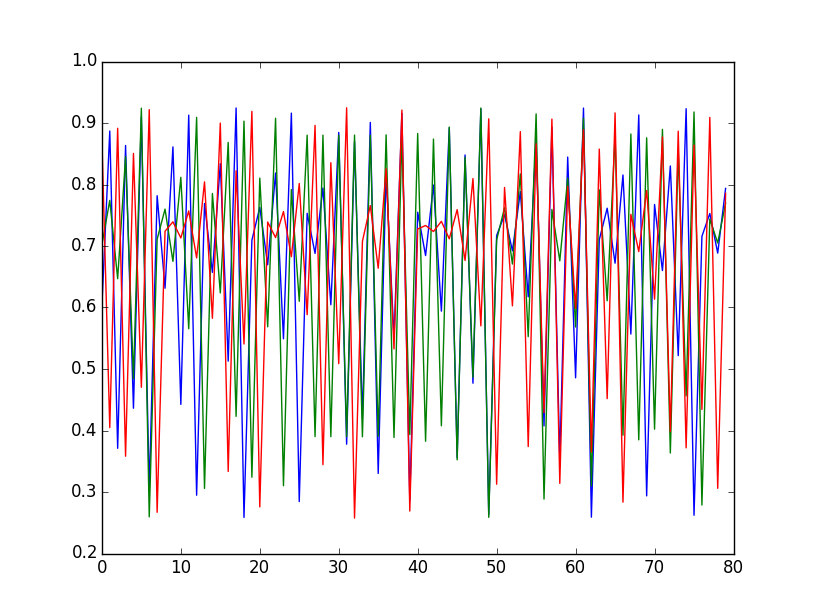
\includegraphics[width = 0.8\textwidth]{population-development2}
\end{figure}
\end{minipage}
\end{tabular}
\end{frame}


\section*{The Lyapunov Exponent}
\begin{frame}
\begin{itemize}
\frametitle{The Lyapunov Exponent}
\item Observing the phase space separation of two trajectories $\delta\Gamma(t)$, we define
\begin{equation}
\left|\delta\Gamma(t)\right|\approx \lim\limits_{\left|\Gamma_0\right| \rightarrow0} e^{\lambda t}\left|\delta\Gamma_0\right|
\end{equation}
\item $\lambda:$ Lyapunov Exponent
\item $\Gamma_0:$ initial phase space seperation (infinitesimal)
\item $\Gamma(t):$ time development of phase space separation 
\begin{equation}
\Leftrightarrow \lambda\approx \lim\limits_{\left|\Gamma_0\right| \rightarrow0} \frac{1}{t}\ln\left|\frac{\delta\Gamma(t)}{\delta\Gamma_0}\right|
\end{equation}
\end{itemize}
\end{frame}

\begin{frame}
\frametitle{Maximal Lyapunov Exponent}
\begin{itemize}
\item Maximal Lyapunov Exponent defined as:
\begin{equation}
\Leftrightarrow \lambda = \lim\limits_{t \rightarrow \infty} \lim\limits_{\left|\Gamma_0\right| \rightarrow0}  \frac{1}{t}\ln\left|\frac{\delta\Gamma(t)}{\delta\Gamma_0}\right|
\end{equation}
\item Considering a discrete one-dimensional system following
\begin{equation}
x_{n+1}=f(x_n)
\end{equation}
\item Lyapunov Exponent
\begin{equation}
\lambda(x_0)=\lim\limits_{N\rightarrow\infty} \frac{1}{N} \ln\left|\frac{\mathrm{d}f^N(x_0)}{\mathrm{d}x}\right|
\end{equation}
\end{itemize}
\end{frame}

\begin{frame}
\frametitle{Maximal Lyapunov Exponent(2)}
\begin{itemize}
\item Using the chain rule
\begin{equation}
\frac{\dif f^N(x_0)}{\dif x}=\frac{\dif (f(f(...f(x_0))))}{\dif x}=
f'(x_N)\cdot f'(x_{N-1})\cdot ...\cdot f'(x_0)=\prod\limits_{n=0}^{N-1} f'(x_n)
\end{equation}
\item Lyapunov Exponent
\begin{equation}
\lambda(x_0)=\lim \limits_{N\rightarrow\infty}\frac{1}{N}\sum\limits_{n=0}^{N-1}\ln|f'(x_n)|
\end{equation}
\item Numerical approximation with finite $N$ 
\end{itemize}
\end{frame}

\begin{frame}
\frametitle{Lyapunov Exponent for Logistic Formula}
\begin{equation}
x_{n+1} = f(x_n)=rx_n(1-x_n)
\end{equation}
\begin{equation}
f'(x_n) = r-2rx_n
\end{equation}
\begin{equation}
\lambda(x_0)= \lim \limits_{N\rightarrow\infty}\frac{1}{N}\sum\limits_{n=0}^{N-1}\ln|r-2rx_n|
\end{equation}
\end{frame}

\section*{Lyapunov Space}
\begin{frame}
\frametitle{Lyapunov Space}
\begin{tabular}{cr}
\begin{minipage}[t]{0.5\textwidth}
\vspace*{5pt}
\begin{itemize}	
\item $r$ not considered fix
\item Instead: $r$ alternates e.g. $a-b-a-b-a-b-...$ with $a,b\in (1,4)$
\item Calculation of Lyapunov Exponent for every pair $(a,b)$ 
\item Every pair $(a,b)$: pixel colored according to Lyapunov Exponent ($>0$: black, $\leq0$: different grade of orange)
\end{itemize}
\end{minipage}

\begin{minipage}[t]{0.4\textwidth}
\begin{figure}[htbp]
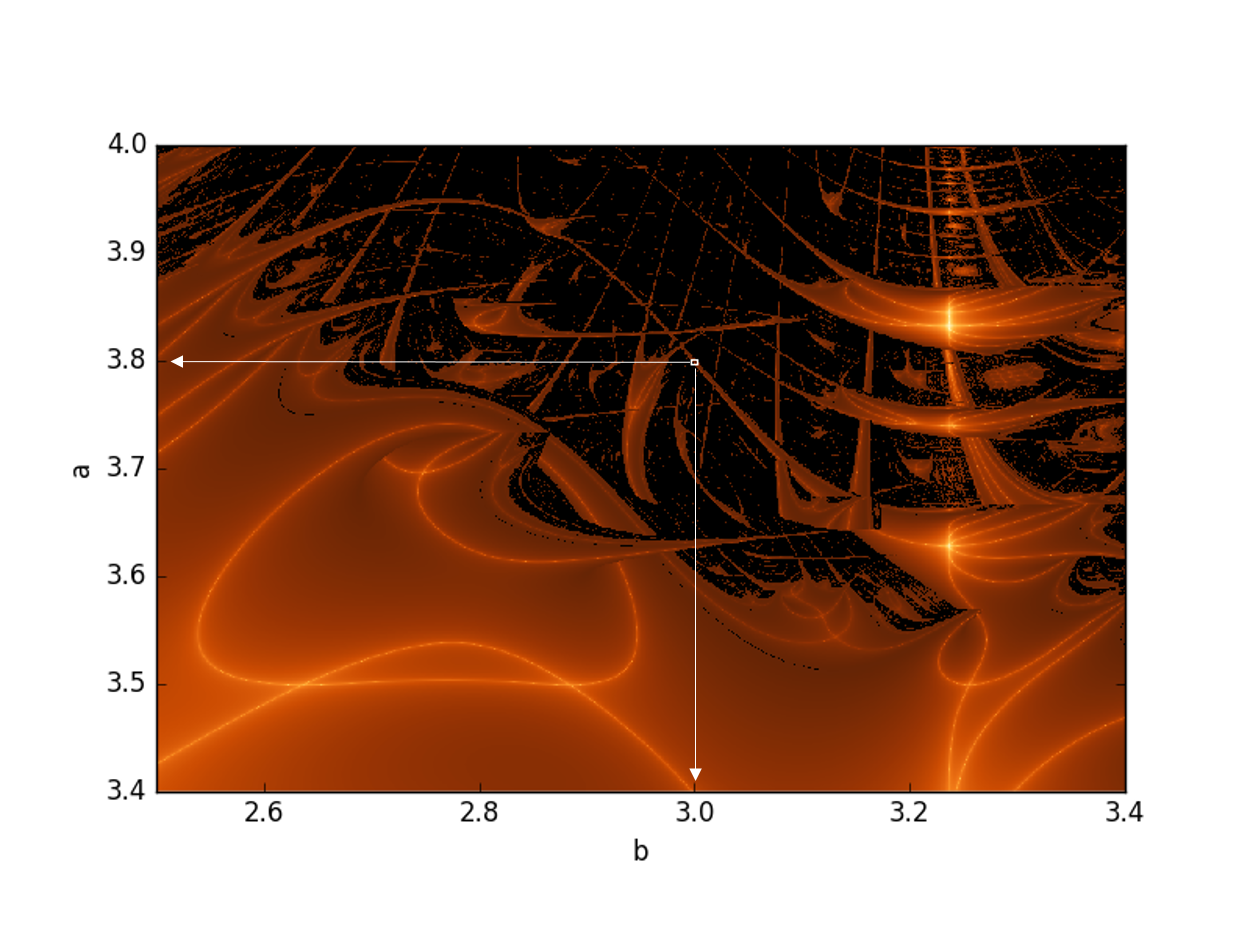
\includegraphics[width = \textwidth]{erklaerung.png}
\end{figure}
\end{minipage}
\end{tabular}
\end{frame}

\section*{Algorithm and Code presentation}
\begin{frame}
\begin{center}
\begin{Huge}
Our Implementation
\end{Huge}
\end{center}
\end{frame}

\begin{frame}
\frametitle{Sequence 'ab': Overview 1.0-4.0}
\begin{figure}[htbp]
\vspace*{5pt}
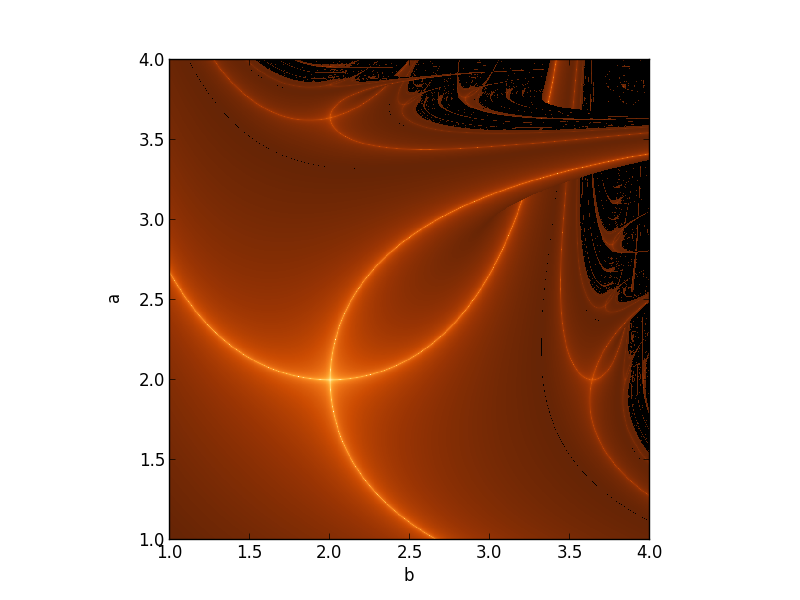
\includegraphics[scale = 0.5]{pictures/Overview_ab.png}
\end{figure}
\end{frame}

\begin{frame}
\frametitle{Sequence 'ab': Self-Similarity(1)}
\begin{figure}[htbp]
\vspace*{5pt}
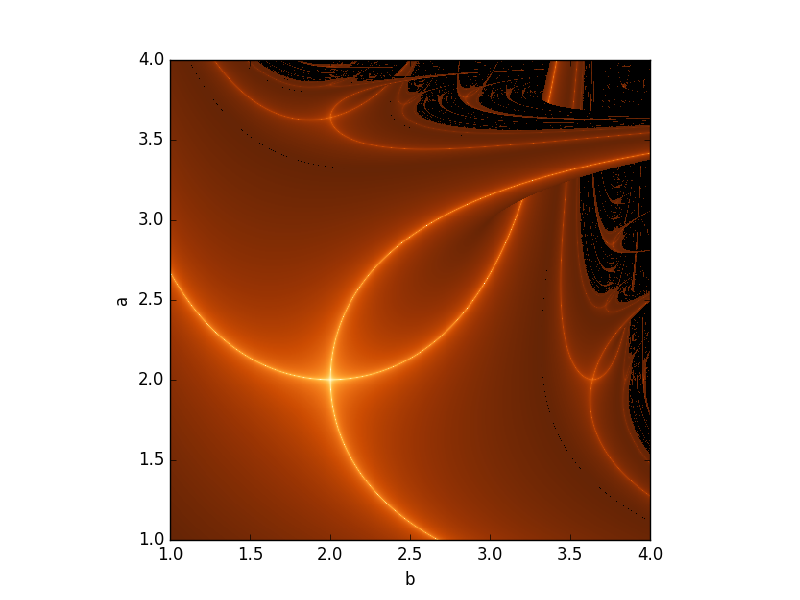
\includegraphics[scale = 0.5]{pictures/ab_selfsim_1.png}
\end{figure}
\end{frame}

\begin{frame}
\frametitle{Sequence 'ab': Self-Similarity(2)}
\begin{figure}[htbp]
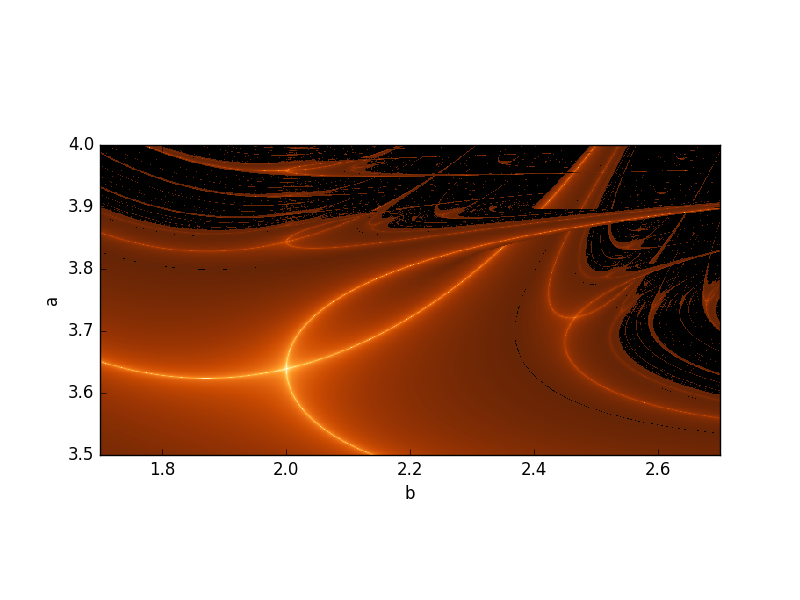
\includegraphics[scale = 0.5]{pictures/ab_selfsim_2.png}
\end{figure}
\end{frame}

\begin{frame}
\frametitle{Sequence 'ab': Self-Similarity(3)}
\begin{figure}[htbp]
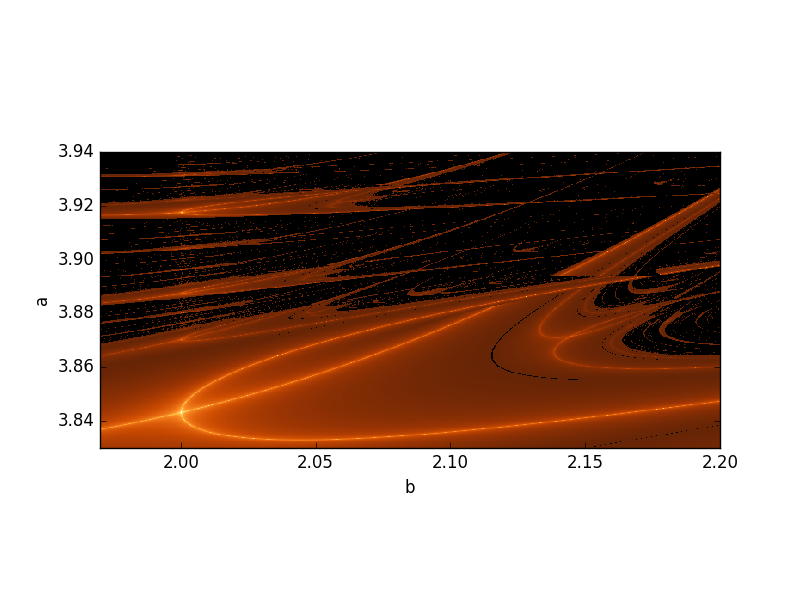
\includegraphics[scale = 0.5]{pictures/ab_selfsim_3.png}
\end{figure}
\end{frame}

\begin{frame}
\frametitle{Sequence 'ab': Lyapunov-Space}
\begin{figure}[htbp]
\vspace*{5pt}
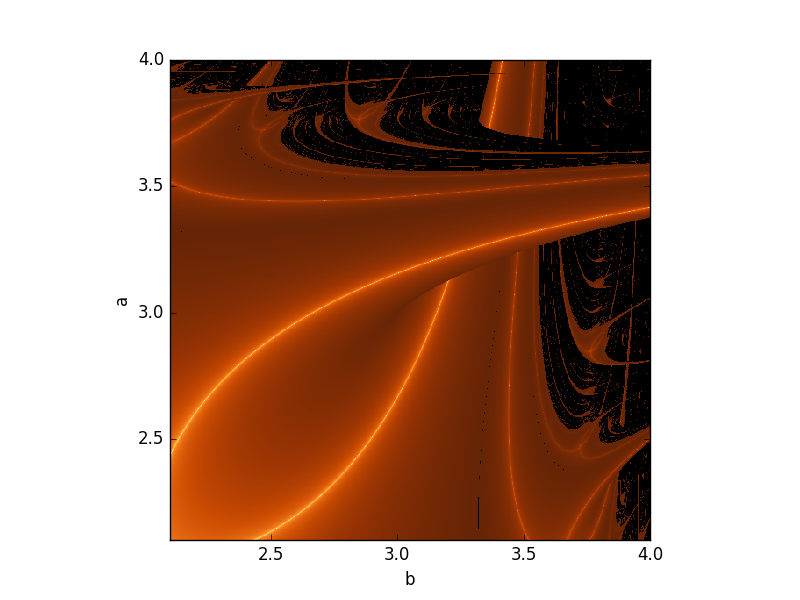
\includegraphics[scale = 0.5]{pictures/ab_lyapunov-space.png}
\end{figure}
\end{frame}

\begin{frame}
\frametitle{Sequence 'ab': The Swallow}
\begin{figure}[htbp]
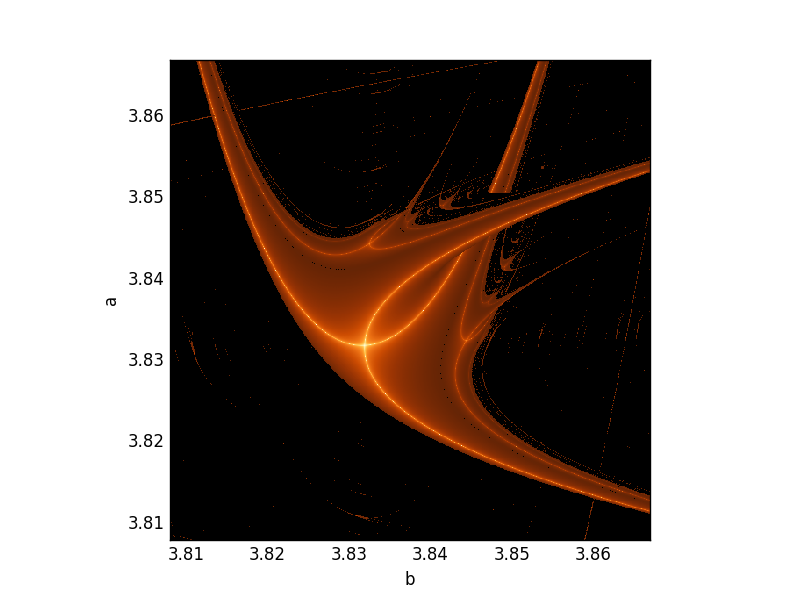
\includegraphics[scale = 0.5]{pictures/The-swallow_ab.png}
\end{figure}
\end{frame}

\begin{frame}
\frametitle{Sequence 'ab': The Swallow Self-Similarity}
\begin{figure}[htbp]
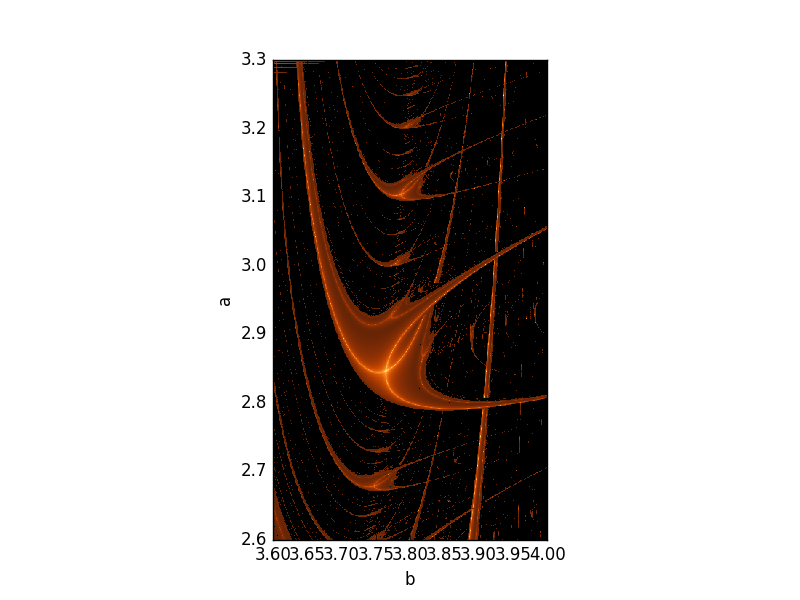
\includegraphics[scale = 0.5]{pictures/The-swallow-ab-self.png}
\end{figure}
\end{frame}

\begin{frame}
\frametitle{Sequence 'bbaba': Overview 1.0-4.0}
\begin{figure}[htbp]
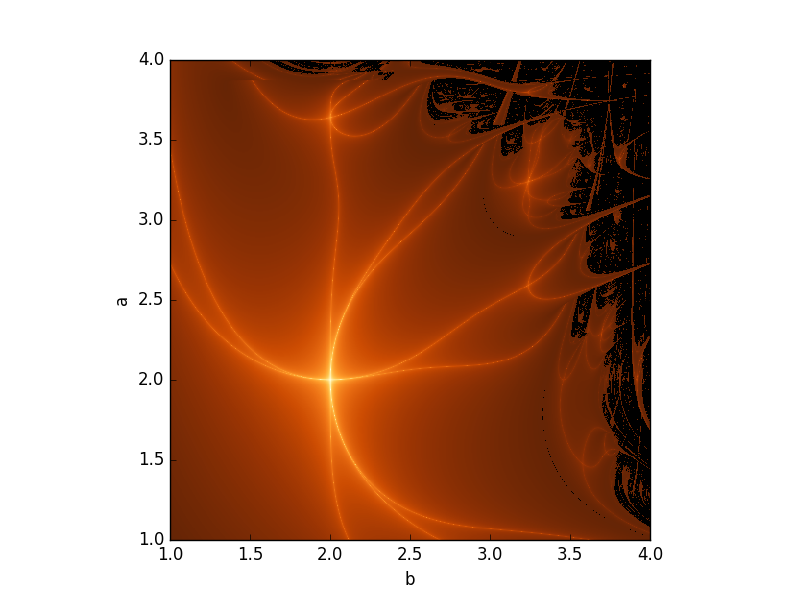
\includegraphics[scale = 0.5]{pictures/Overview_bbaba.png}
\end{figure}
\end{frame}

\begin{frame}
\frametitle{Sequence 'bbaba': Lyapunov Jellyfish}
\begin{figure}[htbp]
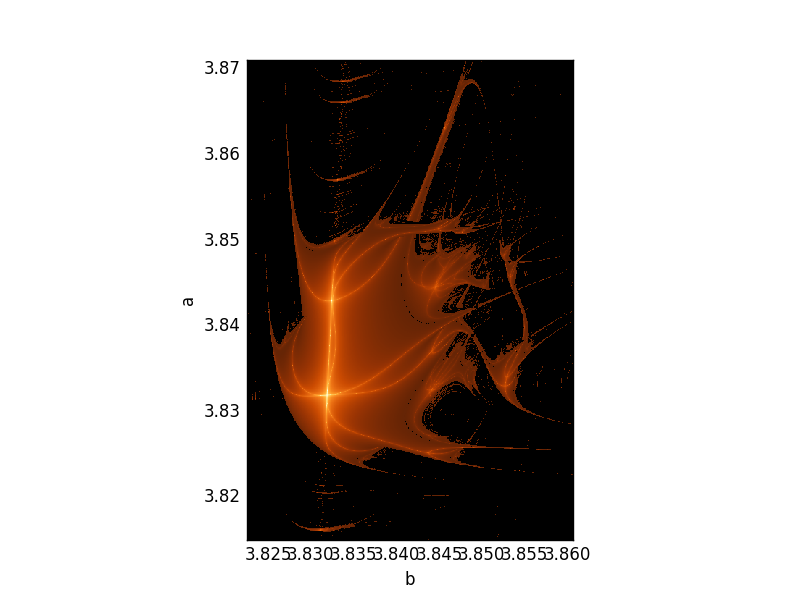
\includegraphics[scale = 0.5]{pictures/bbaba_jellyfish.png}
\end{figure}
\end{frame}

\begin{frame}
\frametitle{Sequence 'bbbbbbaaaaaa': Overview 1.0-4.0}
\begin{figure}[htbp]
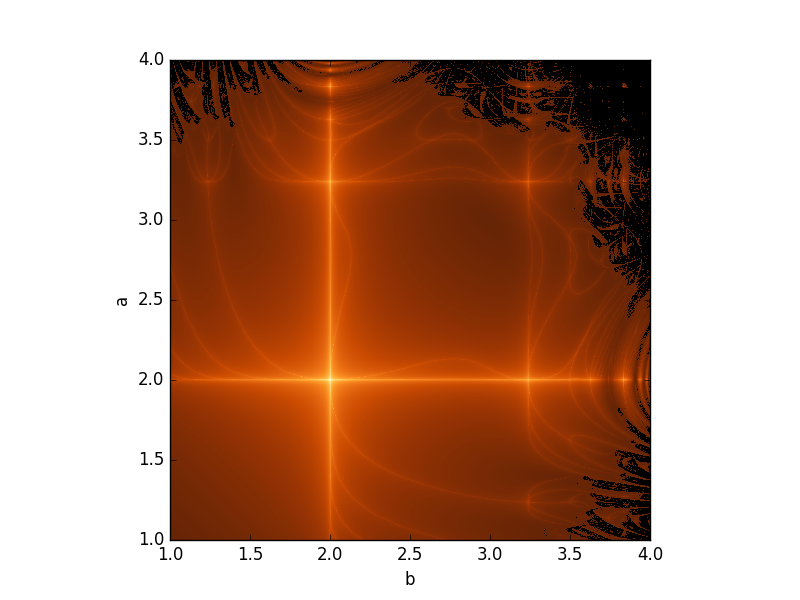
\includegraphics[scale = 0.5]{pictures/Overview_bbbbbbaaaaaa.png}
\end{figure}
\end{frame}

\begin{frame}
\frametitle{Sequence 'bbbbbbaaaaaa': Zircon Zity}
\begin{figure}[htbp]
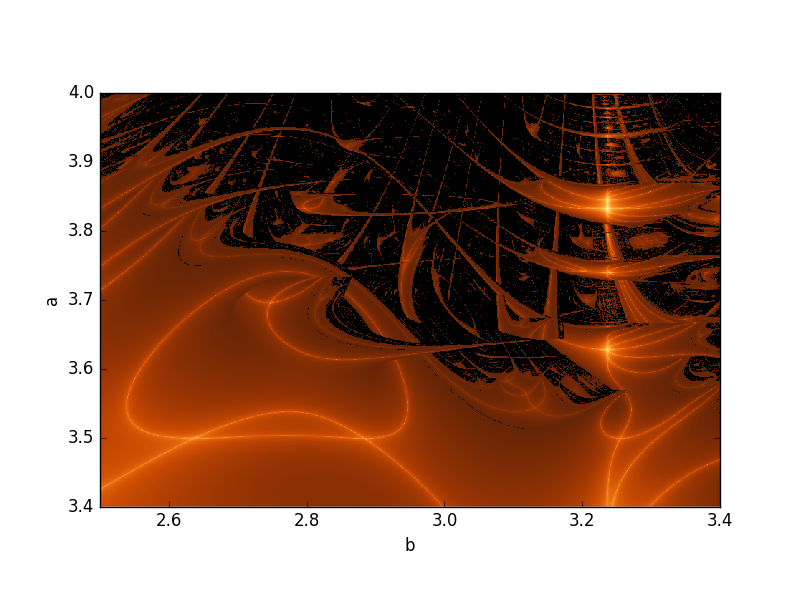
\includegraphics[scale = 0.5]{pictures/zircon_city.png}
\end{figure}
\end{frame}

\begin{frame}
\center{\Huge{Thank you for your attention!}}\\
\center{\large{Presentation and source code:}}\\
\center{\underline{\large{https://github.com/millinma/lyapunov}}}
\end{frame}

\end{document}


